\documentclass[aspectratio=169,professionalfonts]{beamer}
\usetheme{Madrid}
\usecolortheme{default}
\usepackage{booktabs}
\usepackage{tikz}
\usetikzlibrary{arrows.meta,positioning,shapes.geometric}
\definecolor{deepnavy}{RGB}{20,38,70}
\definecolor{accentblue}{RGB}{42,111,219}
\definecolor{softgreen}{RGB}{62,158,120}
\definecolor{warmorange}{RGB}{231,139,47}
\definecolor{lightbg}{RGB}{246,248,252}
\setbeamercolor{title}{fg=white,bg=deepnavy}
\setbeamercolor{frametitle}{fg=white,bg=deepnavy}
\setbeamercolor{block title}{fg=white,bg=accentblue}
\setbeamercolor{block body}{bg=lightbg,fg=black}
\setbeamertemplate{navigation symbols}{}
\setbeamertemplate{footline}[frame number]
\title[Beam Scheduler]{Beam Search Scheduling for DAG Computation Graphs}
\subtitle{Tile-simulated scheduling under limited fast memory}
\author{Wenqi Deng}
\institute{Peking University}
\date{Google MLSys Competition 2026 \\ Track A: Systems Engineering}


\begin{document}
\begin{frame}
  \titlepage
\end{frame}

\begin{frame}{Team and Acknowledgement}
\begin{columns}[c]

% left column
\begin{column}{0.45\textwidth}
\vspace{1em}
\begin{itemize}
    \item \textbf{Presenter: Wenqi Deng}
    \item School of EECS, Peking University
    \item Undergraduate student, Turing Class
\end{itemize}
\vspace{0.8em}
\centering
\includegraphics[
    width=0.6\linewidth,
    height=0.6\textheight,
    keepaspectratio
]{figures/wenqi_deng.png}
\end{column}

% right column
\begin{column}{0.50\textwidth}
\centering
\includegraphics[
    width=0.78\linewidth,
    height=0.48\textheight,
    keepaspectratio
]{figures/xupeng.png}

\vspace{0.6em}

\centering
\textbf{Advisor: Prof. Xupeng Miao}\\
Peking University

\vspace{0.2em}


\begin{block}{Acknowledgement}
I would like to thank Prof. Xupeng Miao for his valuable guidance and support.
\end{block}
\end{column}


\end{columns}
\end{frame}


\begin{frame}{Problem Definition}
\begin{columns}[T]
\begin{column}{0.6\textwidth}
\begin{block}{Objective}
Minimize total latency while every execution step fits in fast memory.
\end{block}
\begin{itemize}
\item Slow memory: large but bandwidth-limited.
\item Fast memory: fast but capacity-limited
\item Fusing ops creates ephemeral internal tensors.
\item Each subgraph is assigned a granularity \([w,h,k]\).
\end{itemize}
\end{column}
\begin{column}{0.35\textwidth}
\centering
\vspace{2em}
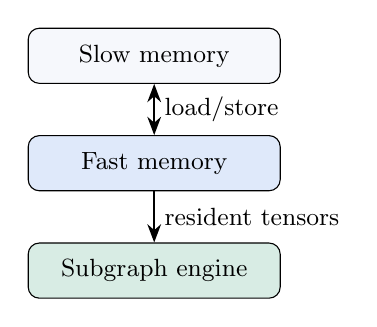
\begin{tikzpicture}[node distance=0.65cm, every node/.style={font=\small}]
\node[draw,rounded corners,fill=lightbg,minimum width=3.2cm,minimum height=0.7cm] (slow) {Slow memory};
\node[draw,rounded corners,fill=accentblue!15,below=of slow,minimum width=3.2cm,minimum height=0.7cm] (fast) {Fast memory};
\node[draw,rounded corners,fill=softgreen!20,below=of fast,minimum width=3.2cm,minimum height=0.7cm] (sub) {Subgraph engine};
\draw[{Stealth}-{Stealth},thick] (slow) -- node[right]{load/store} (fast);
\draw[-{Stealth},thick] (fast) -- node[right]{resident tensors} (sub);
\end{tikzpicture}
\end{column}
\end{columns}
\end{frame}

\begin{frame}{Search Model}
\begin{block}{Search state representation}
\[
State(\text{covered ops},\ \text{stored tensors},\ \text{resident tensors})
\]
\end{block}
\begin{columns}[c]
\begin{column}{0.30\textwidth}
\begin{itemize}
\item Start: graph inputs are stored in slow memory.
\item Transition: choose one feasible subgraph.
\item Goal: all ops covered and outputs stored.
\end{itemize}
\end{column}
\begin{column}{0.7\textwidth}

\includegraphics[
    width=1\linewidth,
    height=0.6\textheight,
    keepaspectratio
]{figures/search-model.png}
\end{column}
\end{columns}
\end{frame}


\begin{frame}{Beam Search Loop}
\begin{enumerate}
\item Expand each beam state with generated candidates.
\item Evaluate each candidate through the simulator.
\item Append the chosen subgraph to form a next state.
\item Deduplicate equivalent states.
\item Keep the best states by estimated total latency.
\end{enumerate}
\begin{block}{Priority function}
\[
\text{priority}(State)=\text{latency}(State)+0.1\times\sum_{\text{uncovered ops}}\text{base\_cost}
\]
\end{block}
\end{frame}

\begin{frame}{Candidate Generation}
\begin{columns}[T]
\begin{column}{0.52\textwidth}
\begin{itemize}
\item Ready single operations.
\item Linear pointwise chains.
\item Pointwise backward cones.
\item Shallow recomputation cones.
\end{itemize}
\begin{block}{Design principle}
Generate a small set of high-value subgraph templates, then let the evaluator reject illegal or expensive ones.
\end{block}
\end{column}
\begin{column}{0.42\textwidth}
\centering
\vspace{1em}
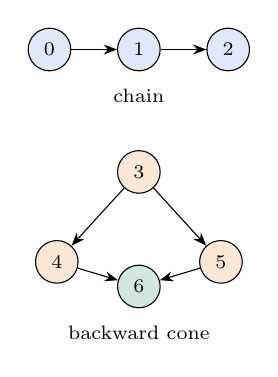
\begin{tikzpicture}[node distance=0.58cm, every node/.style={font=\scriptsize}]
\node[draw,circle,fill=accentblue!15] (a) {0};
\node[draw,circle,fill=accentblue!15,right=of a] (b) {1};
\node[draw,circle,fill=accentblue!15,right=of b] (c) {2};

\draw[-{Stealth}] (a)--(b);
\draw[-{Stealth}] (b)--(c);

\node[below=0.1cm of b] {chain};

% backward cone: one source, fan out, then merge into sink op
\node[draw,circle,fill=warmorange!20,below=1.0cm of b] (src) {3};

\node[draw,circle,fill=warmorange!20,below left=0.75cm and 0.65cm of src] (u) {4};
\node[draw,circle,fill=warmorange!20,below right=0.75cm and 0.65cm of src] (v) {5};

\node[draw,circle,fill=softgreen!25,below=0.9cm of src] (sink) {6};

\draw[-{Stealth}] (src) -- (u);
\draw[-{Stealth}] (src) -- (v);
\draw[-{Stealth}] (u) -- (sink);
\draw[-{Stealth}] (v) -- (sink);

\node[below=0.1cm of sink] {backward cone};
\end{tikzpicture}

\end{column}
\end{columns}
\end{frame}

\begin{frame}{Candidate Evaluation}
\begin{center}
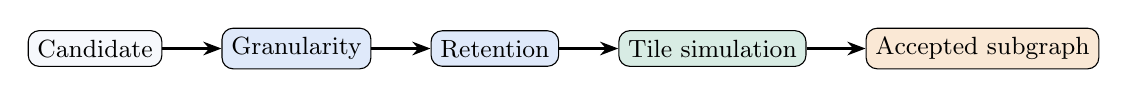
\begin{tikzpicture}[node distance=0.75cm, every node/.style={font=\small}]
\node[draw,rounded corners,fill=lightbg] (c) {Candidate};
\node[draw,rounded corners,fill=accentblue!15,right=of c] (g) {Granularity};
\node[draw,rounded corners,fill=accentblue!15,right=of g] (r) {Retention};
\node[draw,rounded corners,fill=softgreen!20,right=of r] (sim) {Tile simulation};
\node[draw,rounded corners,fill=warmorange!20,right=of sim] (best) {Accepted subgraph};
\draw[-{Stealth},thick] (c)--(g);
\draw[-{Stealth},thick] (g)--(r);
\draw[-{Stealth},thick] (r)--(sim);
\draw[-{Stealth},thick] (sim)--(best);
\end{tikzpicture}
\end{center}
\begin{itemize}
\item Enumerate \(w,h\) choices, and choose the largest available \(k\).
\item Enumerate retain sets on boundary outputs.
\item Reject any combination with an OOM step.
\item Return the lowest-latency feasible subgraph.
\end{itemize}
\end{frame}

\begin{frame}{Tile Simulator}
\begin{itemize}
\item Trace required tensor rectangles from the subgraph tip tensor.
\item Track external inputs, boundary outputs, retained tensors and accumulators.
\item Use rectangle union area per tensor to avoid double counting.
\item Validate every spatial tile and every split-k step.
\end{itemize}
\begin{block}{Capacity rule for OOM correctness}
\[
|R_{\text{resident}}\cup R_{\text{retain}}\cup
R_{\text{input}}\cup R_{\text{output}}\cup R_{\text{accumulator}}|
\leq C_{\text{fast}}
\]
\end{block}
\end{frame}


\begin{frame}{Retention}
\begin{block}{Retention is inter-subgraph persistence}
Only selected boundary outputs stay in fast memory for the next scheduling step.
\end{block}
\begin{itemize}
\item Retain candidates are boundary outputs with future consumers.
\item Non-retained boundary outputs are stored back to slow memory.
\item Residents tensors must be consumed at the immediate following tensor.
\end{itemize}
\end{frame}

\begin{frame}{Validation Results}
\begin{table}
\centering
\small
\begin{tabular}{lrr}
\toprule
Benchmark & Latency & Peak fast memory \\
\midrule
mlsys-2026-1 & 471,501 & 49,152 \\
mlsys-2026-5 & 961,195 & 24,576 \\
mlsys-2026-9 & 167,530,988 & 49,152 \\
mlsys-2026-13 & 166,408,847 & 65,536 \\
mlsys-2026-17 & 46,386,493 & 311,296 \\
\bottomrule
\end{tabular}
\end{table}
\begin{block}{Verification}
Solutions were validated on the public benchmarks with our verifier, and the reported latencies are computed by our cost model.
\end{block}
\end{frame}

\begin{frame}{Takeaways}
\begin{itemize}
\item Beam search avoids one-step greedy decisions.
\item Candidate templates keep the search space manageable.
\item Tile simulation gives robust OOM rejection.
\item Retention reduces slow-memory traffic while preserving physical state semantics.
\end{itemize}
\begin{block}{Potential improvements}
Richer MatMul-chain candidates, memory-aware heuristics, and stronger retention scoring.
\end{block}
\end{frame}

\end{document}
